\documentclass[]{article}
\usepackage{amsmath,amssymb}
\usepackage{graphicx}

\usepackage[utf8]{inputenc}
\usepackage[T1]{fontenc}
\usepackage[russian]{babel}


\usepackage{xcolor}
\usepackage{hyperref}
%\usepackage{autonum}
\renewcommand{\[}{\begin{equation}}
\renewcommand{\]}{\end{equation}}

%opening
\title{О полном базисе  в пространстве \\ вращательно-инвариантных операторов \\ $N$ квантовых спинов $1/2$}
\author{Филипп Усков, fe1992@mail.ru\\ {\small Сколковский Институт Науки и Технологий}\\
{\small Большой бульвар д.30, стр.1,
Москва 121205}
\footnote{
Работа выполнена при поддержке Российского Фонда Фундаментальных Исследований, грант № 18-32-20218.
}
}


\begin{document}

\maketitle

\begin{abstract}
В физике большую роль играют системы квантовых спинов $1/2$ с изотропным гейзенберговским взаимодействием. При изучении таких систем может быть полезно иметь полный, но не переполненный базис операторов, каждый из которых имеет симметрию гамильтониана, то есть инвариантен относительно вращений (т.е. глобальных $SU(2)$-преобразований матриц Паули).	
%\show \TeX
В настоящей статье сформулирован алгоритм построения такого базиса. Алгоритм реализован в программе Wolfram Mathematica\textsuperscript{\textcopyright}.

{\bf Ключевые слова}: матрицы Паули, изотропное гейзенберговское взаимодействие, системы квантовых спинов, операторный базис.
\end{abstract}

%%%%%%%%%%%%%%%%%%%%%%%%%%%%%%%%%%%%%%%%%%%%%%%%%%%%%%%%%%%%%%%%%%%%
%%%%%%%%%%%%%%%%%%%%%%%%%%%%%%%%%%%%%%%%%%%%%%%%%%%%%%%%%%%%%%%%%%%%
%%%%%%%%%%%%%%%%%%%%%%%%%%%%%%%%%%%%%%%%%%%%%%%%%%%%%%%%%%%%%%%%%%%%
\section{Введение}

В квантовой физике важную роль играют системы $N$ спинов $1/2$ с изотропным гейзенберговским взаимодействием. Общий вид гамильтониана такой системы имеет вид
$$
H=\sum_{i< j}J_{ij}\,(\vec\sigma_i\vec\sigma_j),
%\label{k1}
$$
где $\vec\sigma_i = \{\sigma_i^x,\sigma_i^y,\sigma_i^z\}$ - вектор матриц Паули, $J_{ij}$ - константы связи,   индексы $i,j=1,2,...,N$ нумеруют спины, а $(\vec\sigma_i\vec\sigma_j)\equiv \sigma_i^\alpha \sigma_j^\alpha$ -- скалярное произведение векторов сигма-матриц (здесь и далее предполагается суммирование по повторяющимся индексам).

Состояние квантовой  систмемы описаывается в общем случае матрицей плотности $\rho$. Зачастую, в силу симметрии гамильтониана относительно глобальных вращений, такой же симметрией должна обладать и матрица плотности. Это справедливо, например, когда необходимо решить стационарное уравнение Шредингера, записанное в виде $ H\rho = E\rho $ \cite{USH}, или при поиске вариационных ограничений на энергию основного состояния \cite{variational} с использованием квадратичной параметризации матрицы плотности \cite{kvadro}.   Также нередки случаи, когда необходимо записать вращательно-инвариантный оператор общего вида (не обязательно матрицу плотности) -- например, для нахождения интегралов движения \cite{basisF} или доказательства их отсутствия \cite{Shiraishi}, а также для конструирования приближенных интегралов движения в неинтегрируемых системах \cite{Malikis}.  

Простой способ соблюсти условие вращательной инвариантности оператора -- представить его в виде суммы слагаемых, каждое из которых является произведением скалярных и смешанных произведений матриц Паули (или единичным оператором). Например, для $N=4$ спинов любой вращательно-инвариантный оператор можно разложить по следующему операторному базису:
\begin{align}
\{ & 1,  \;\;
({\vec \sigma}_1{\vec\sigma}_2), \;\; 
({\vec \sigma}_2{\vec\sigma}_3), \;\;
({\vec \sigma}_3{\vec\sigma}_4), \;\;
({\vec \sigma}_1{\vec\sigma}_3), \;\;
({\vec \sigma}_2{\vec\sigma}_4), \;\;
({\vec \sigma}_1{\vec\sigma}_4), \;\;
\nonumber\\
&({\vec \sigma}_1{\vec\sigma}_2)({\vec \sigma}_3{\vec\sigma}_4),\;\;({\vec \sigma}_1{\vec\sigma}_3)({\vec \sigma}_2{\vec\sigma}_4),\;\;
({\vec \sigma}_1{\vec\sigma}_4)({\vec \sigma}_2{\vec\sigma}_3),\;\; \nonumber \\
&({\vec \sigma}_1{\vec\sigma}_2{\vec\sigma}_3),\;\;({\vec \sigma}_1{\vec\sigma}_2{\vec\sigma}_4),\;\;({\vec \sigma}_2{\vec\sigma}_3{\vec\sigma}_4)
\},
\label{k2}
\end{align}
где $({\vec \sigma}_i{\vec\sigma}_j{\vec\sigma}_k)\equiv \varepsilon_{\alpha \beta \gamma} \, \sigma_i^\alpha \sigma_j^\beta \sigma_k^\gamma$ обозначает смешанное поизведение матриц Паули ($ \varepsilon_{\alpha \beta \gamma}$  -- антисимметричный тензор).
При этом даже для большего числа спинов в каждом элементе базиса не должно быть больше одного смешанного произведения, т.к. произведение двух смешанных произведений раскладывается в полином из скалярных произведений благодаря тождеству
\[
(\vec\sigma_1,\vec\sigma_2,\vec\sigma_3)
(\vec\sigma_4,\vec\sigma_5,\vec\sigma_6)=
\begin{vmatrix}
	(\vec\sigma_1,\vec\sigma_4) & 	(\vec\sigma_1,\vec\sigma_5) & (\vec\sigma_1,\vec\sigma_6) \\
	(\vec\sigma_2,\vec\sigma_4) & 	(\vec\sigma_2,\vec\sigma_5) & (\vec\sigma_2,\vec\sigma_6) \\
	(\vec\sigma_3,\vec\sigma_4) & 	(\vec\sigma_3,\vec\sigma_5) & (\vec\sigma_3,\vec\sigma_6) \\
\end{vmatrix}.
\label{k3}
\]
Заметим еще, что если потребовать инвариантности оператора относительно обращения по времени (преобразование $\vec\sigma_i\rightarrow -\sigma_i$), то в базисе следует оставить только элементы без смешанного произведения.


Недостатком базиса типа \eqref{k2} является его переполненность для $N\geq 5$ \cite{variational}(пример линейной зависимости см. в ур. \eqref{k10}).
В настоящей статье, опираясь на результаты работы \cite{sourceArticle}, мы опишем алгоритм построения полного, но не переполненного операторного базиса, каждый элемент которого вращательно-инвариантен.

%%%%%%%%%%%%%%%%%%%%%%%%%%%%%%%%%%%%%%%%%%%%%%%%%%%%%%%%%%%%%%%%%%%%
%%%%%%%%%%%%%%%%%%%%%%%%%%%%%%%%%%%%%%%%%%%%%%%%%%%%%%%%%%%%%%%%%%%%
%%%%%%%%%%%%%%%%%%%%%%%%%%%%%%%%%%%%%%%%%%%%%%%%%%%%%%%%%%%%%%%%%%%%
%\section{Цель и ход работы}
%Мы захотели получить этот базис в непереполненном виде, чтобы немного сократить объем вычилений.

%Мы нашли статью \cite{basis_f} про "базис f", но через год, когда мы ее всё-таки прочитали, оказалось что это вообще не имеет ни какого отношения к нашему базису.

%Мы решили посчитать сколько же на самом деле линейнонезависимых векторов в нашем базисе для небольшого числа спинов,
%нашли эту последовательность на OEIS,
%и нашли статью, которая описывает, как строить непереполненный базис, и вот что там говориться:

%%%%%%%%%%%%%%%%%%%%%%%%%%%%%%%%%%%%%%%%%%%%%%%%%%%%%%%%%%%%%%%%%%%%
%%%%%%%%%%%%%%%%%%%%%%%%%%%%%%%%%%%%%%%%%%%%%%%%%%%%%%%%%%%%%%%%%%%%
%%%%%%%%%%%%%%%%%%%%%%%%%%%%%%%%%%%%%%%%%%%%%%%%%%%%%%%%%%%%%%%%%%%%
\section{Построение непереполненного базиса}
\subsection{Таблички}
Следуя \cite{sourceArticle}, каждому элементу базиса поставим в соответствие {\it табличку}. Эти таблички заполняются номерами спинов.

Столбец высоты 3 мы интерпретируем как смешанное произведение.
$$
\begin{tabular}{ | l | }
\hline
1 \\ \hline
2 \\ \hline
3 \\
\hline
\end{tabular} = (\vec \sigma_1, \vec \sigma_2, \vec \sigma_3)
%\label{k4}
$$
Пару столбцов мы интерпретируем как определитель, составленный из скалярных произведений (или, что то же самое, обобщенный символ Кронекера\cite{kronecker_wiki}, свёрнутый со всеми векторами сигма-матриц), например
$$
\begin{tabular}{ |l|l| }
\hline
1 & 4 \\ \hline
2 & 5\\
\hline
\end{tabular}
 =
 \sigma_1^{\alpha_1} \sigma_2^{\alpha_2}
 (\delta_{\alpha_1\alpha_2}^{\alpha_4\alpha_5})
 \sigma_4^{\alpha_4} \sigma_5^{\alpha_5}
 =
\begin{vmatrix}
(\vec\sigma_1,\vec\sigma_4) & (\vec\sigma_1,\vec\sigma_5)\\
(\vec\sigma_2,\vec\sigma_4) & (\vec\sigma_2,\vec\sigma_5)\\
\end{vmatrix}.
%\label{k5}
$$
Пара столбцов высоты 1 -- это просто скалярное произведение
$$
\begin{tabular}{ |l|l| }
\hline
1 & 2 \\
\hline
\end{tabular}
= (\vec \sigma_1, \vec \sigma_2).
%\label{k6}
$$
Заметим, что по этому правилу пара столбцов высоты 3 равна произведению двух смешанных произведений (каждое соответствует  своему столбцу), и мы воспроизводим ур. \eqref{k3}:
\begin{align}
\begin{tabular}{ |l|l| }
\hline
1 & 4 \\ \hline
2 & 5\\ \hline
3 & 6\\
\hline
\end{tabular}
=
\begin{vmatrix}
(\vec\sigma_1,\vec\sigma_4) & (\vec\sigma_1,\vec\sigma_5) & (\vec\sigma_1,\vec\sigma_6) \\
(\vec\sigma_2,\vec\sigma_4) & (\vec\sigma_2,\vec\sigma_5) & (\vec\sigma_2,\vec\sigma_6) \\
(\vec\sigma_3,\vec\sigma_4) & (\vec\sigma_3,\vec\sigma_5) & (\vec\sigma_3,\vec\sigma_6) \\
\end{vmatrix}
=\nonumber\\
=
(\vec \sigma_1, \vec \sigma_2, \vec \sigma_3)
(\vec \sigma_4, \vec \sigma_5, \vec \sigma_6)
=
\begin{tabular}{ |l| }
\hline
1  \\ \hline
2 \\ \hline
3 \\
\hline
\end{tabular}
\;\;
\begin{tabular}{ |l| }
\hline
 4 \\ \hline
 5\\ \hline
 6\\
\hline
\end{tabular}
.\nonumber
%\label{k7}
\end{align}

Таблички из большего количества столбцов разбивается на пары столбцов с конца. При этом в начале может остаться 1 столбец. Например:
%\tracingcommands=1
$$
{
		\begin{tabular}{ | l | }
		\hline
		1 \\ \hline
		2 \\ \hline
		3 \\
		\hline
		\end{tabular}
	\kern -3.5pt
	\raise 6.2pt \hbox
	{
		\begin{tabular}{ |l|l| }
		\hline
		4 & 6 \\ \hline
		5 & 7\\
		\hline
		\end{tabular}
	}
	\kern -6.5pt
	\raise 12.4pt \hbox
	{
		\begin{tabular}{ |l|l| }
		\hline
		8 & 9 \\
		\hline
		\end{tabular}
	}
}
=
\begin{tabular}{ | l | }
\hline
1 \\ \hline
2 \\ \hline
3 \\
\hline
\end{tabular}
\cdot
\begin{tabular}{ |l|l| }
\hline
4 & 6 \\ \hline
5 & 7\\
\hline
\end{tabular}
\cdot
\begin{tabular}{ |l|l| }
\hline
8 & 9 \\
\hline
\end{tabular}
%\label{manytable}
$$
%\tracingcommands=0

\subsection{Алгоритм построения базиса}

Следуя \cite{sourceArticle}, рассмотрим построение базиса для $N$ спинов. Этот базис включает в себя единичный оператор, а также операторы с $n=2,3,\dots N$ матрицами Паули. Для фиксированного $n$ в базис  войдут элементы, удовлетворяющие следующим критериям:
\begin{itemize}
    \item полное число ячеек в табличке равно $n$
	\item каждая строка в табличке содержит число ячеек не больше, чем в предыдущей строке
	\item строк не больше 3
	\item Для четного числа спинов:
	\begin{itemize}
		\item столбцы разбиваются на пары, высоты столбцов в каждой паре совпадают
	\end{itemize}
	\item Для нечетного числа спинов:
	\begin{itemize}
		\item в начале таблички добавляется столбец высоты 3
		\item оставшиеся $n-3$ ячейки строятся как для четного числа спинов
	\end{itemize}


Для пояснения этих шагов, приведем примеры допустимых {\it форм} табличек:
	
		%\hsize = 18em
	\begin{tabular}{ |c|l| }
		\hline
		$n$ (число матриц Паули)  &  допустимые формы табличек\\
		\hline
		2 & 
		{ \hsize=15em
		\vbox{
			\vskip 1pt
			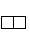
\includegraphics{1x2.png}
			%\vskip 1pt
		}}
		\\ \hline
		3 &
		{ \hsize=15em
		\vbox{
			\vskip 1pt
			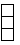
\includegraphics{3x1.png}
		}}
		\\ \hline
		4 &
		{ \hsize=15em
		\vbox{
			\vskip 1pt
			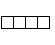
\includegraphics{1x4.png}
			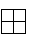
\includegraphics{2x2.png}
		}}
		\\ \hline
		5 &
		{ \hsize=15em
		\vbox{
			\vskip 1pt
			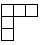
\includegraphics{3x3.png}
		}}
		\\ \hline
		6 &
		{ \hsize=15em
		\vbox{
			\vskip 1pt
			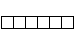
\includegraphics{1x6.png}
			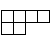
\includegraphics{2x4.png}
			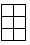
\includegraphics{3x2.png}
		}}
		\\ \hline
		7 &
		{ \hsize=15em
		\vbox{
			\vskip 1pt
			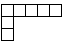
\includegraphics{3x5.png}
			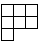
\includegraphics{3x3(7).png}
		}}
		\\ \hline
		8 &
		{ \hsize=18em
		\vbox{
			\vskip 1pt
			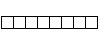
\includegraphics{1x8.png}
			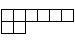
\includegraphics{2x6.png}
			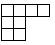
\includegraphics{3x4.png}
		}}
		\\ \hline
	\end{tabular}

	\item заполняем эти таблички различающимися номерами спинов так, чтобы каждая строка и каждый столбец был отсортирован по возрастанию номера спина (вообще говоря, правило сортировки может быть любым, но его нужно придерживаться для всех элементов базиса)

	
	Примеры заполнения одной таблички:
$$
\begin{tabular}{ |l|l|l|l| }
\hline
1 & 2 \\ \hline
3 & 4 \\ \hline
5 & 6 \\
\hline
\end{tabular}
	\quad	
\begin{tabular}{ |l|l|l|l| }
\hline
1&2 \\ \hline
3&5 \\ \hline
4&6 \\
\hline
\end{tabular}
	\quad	
\begin{tabular}{ |l|l|l|l| }
\hline
1&3 \\ \hline
2&4 \\ \hline
5&6 \\
\hline
\end{tabular}
	\quad	
\begin{tabular}{ |l|l|l|l| }
\hline
1&3 \\ \hline
2&5 \\ \hline
4&6 \\
\hline
\end{tabular}
	\quad	
\begin{tabular}{ |l|l|l|l| }
\hline
1&4 \\ \hline
2&5 \\ \hline
3&6 \\
\hline
\end{tabular}
%\label{k8}
$$
\end{itemize}



Например, для $n=4$ матриц Паули мы получим три элемента
\begin{align}
\begin{tabular}{ |l|l|l|l| }
\hline
1 & 2 & 3 & 4 \\
\hline
\end{tabular} & = ({\vec \sigma}_1{\vec\sigma}_2)({\vec \sigma}_3{\vec\sigma}_4), \nonumber
\\
%	
\begin{tabular}{ |l|l| }
\hline
1 & 2 \\ \hline
3 & 4 \\
\hline
\end{tabular} &
=\begin{vmatrix}
(\vec\sigma_1,\vec\sigma_2) & (\vec\sigma_1,\vec\sigma_4)\\
(\vec\sigma_3,\vec\sigma_2) & (\vec\sigma_3,\vec\sigma_4)\\
\end{vmatrix}, \nonumber
\\
%
\begin{tabular}{ |l|l| }
\hline
1 & 3 \\ \hline
2 & 4 \\
\hline
\end{tabular} &
=\begin{vmatrix}
(\vec\sigma_1,\vec\sigma_3) & (\vec\sigma_1,\vec\sigma_4)\\
(\vec\sigma_2,\vec\sigma_3) & (\vec\sigma_2,\vec\sigma_4),\\
\end{vmatrix},
\nonumber
%\label{example4}
\end{align}
ср. со второй строкой ур. \eqref{k2}.


Этот алгоритм реализован нами в программе Wolfram Mathematica\textsuperscript{\textcopyright}, а именно  написана функция  \cite{basis_gen_code}, которая генерирует все возможные элементы базиса.

Число элементов базиса с $n$ матрицами Паули дается формулой \cite{sourceArticle}
$$
Q_n = \sum_{r=0}^{[n/2]}\frac{n!(3r-n+1)}{(n-2r)!r!(r+1)!}.
%\label{k9}
$$
Это совпадает с результатом работы функции \cite{basis_gen_code}.


\subsection{Линейные зависимости и сравнение с переполненным базисом}

Ранее нами было замечено \cite{variational}, что оператор, соответсвующий паре столбцов высоты 4, равен нулю, то есть имеет место линейная зависимость
\[
\begin{tabular}{ |l|l| }
\hline
1 & 5 \\ \hline
2 & 6\\ \hline
3 & 7\\ \hline
4 & 8\\
\hline
\end{tabular}
=
\begin{vmatrix}
(\vec\sigma_1,\vec\sigma_5) & (\vec\sigma_1,\vec\sigma_6) & (\vec\sigma_1,\vec\sigma_7) & (\vec\sigma_1,\vec\sigma_8)\\
(\vec\sigma_2,\vec\sigma_5) & (\vec\sigma_2,\vec\sigma_6) & (\vec\sigma_2,\vec\sigma_7) & (\vec\sigma_2,\vec\sigma_8)\\
(\vec\sigma_3,\vec\sigma_5) & (\vec\sigma_3,\vec\sigma_6) & (\vec\sigma_3,\vec\sigma_7) & (\vec\sigma_3,\vec\sigma_8)\\
(\vec\sigma_4,\vec\sigma_5) & (\vec\sigma_4,\vec\sigma_6) & (\vec\sigma_4,\vec\sigma_7) & (\vec\sigma_4,\vec\sigma_8)\\
\end{vmatrix}
=0 .
\label{k10}
\]
Была высказана гипотеза \cite{variational},  что все линейные зависимости в базисе с четным числом спинов имеют аналогичную структуру.

Общее число элементов исходного переполненного базиса с заданным колическтвом матриц Паули, $n$, дается формулой
$$
T_n=\begin{cases}
\frac{n!}{2^{n/2}(n/2)!} & (n=2k)\\
\frac{n!}{3 \cdot 2^{(n-1)/2}((n-3)/2)!} & (n=2k+1)
\end{cases}
%\label{k11}
$$
Было замечено, что если для четного числа спинов сгененрировать все возможные таблички с заданным количеством ячеек $n$, но без ограничения числа строк,
то их общее число оказалось равно $T_n$. Это подкрепляет гипотезу, что все таблички, у которых число строк больше 4 (они соответствуют линейным комбинациям, равным нулю), дают все линейные зависимости в исходном базисе.
Для нечетного количества спинов аналогичный факт нами не установлен.

Поучительно сравнить размеры  переполненного и не переполненного базисов:

\bigskip

\noindent
\begin{tabular}{ |l|l l l l l l l l l l l l l| }
	\hline
	$n$   & 2 & 3 & 4 & 5  & 6  & 7   & 8   & 9    & 10  & 15    & 20 & 30     & 40
	\\ \hline
	$T_n$ & 1 & 1 & 3 & 10 & 15 & 105 & 105 & 1260 & 945 & 4.7E6 & 6.5E8 & 6.2E15 & 3.2E23
	\\ %\hline
	$Q_n$ & 1 & 1 & 3 & 6  & 15 & 36  & 91  & 232  & 603 & 83097 & 1.3E7  & 4.4E11 & 1.7E16
	\\ \hline
\end{tabular}

\bigskip

%
\noindent Из этого сравнения видно, что не переполненный базис значительно меньше.

\section{Заключение}
Мы сформулировали и реализовали алгоритм построения полного, но не переполненного базиса в пространстве операторов системы $N$ спинов $1/2$, инвариантных относительно глобальных вращений системы координат.  Число элементов этого базиса значтельно меньше числа элементов наивного переполненного базиса, сконструированного из всевозможных мономов из скалярных и векторных произведений матриц Паули.

Полученный базис может быть использован для различных задач квантовой физики спиновых систем с изотропным гейзенберговским взаимодействием \cite{USH,variational,kvadro,basisF}.  Заметим, что для многих приложений желательно найти эффективный алгоритм умножения элементов базиса друг на друга (и разложения по этому базису). Этот вопрос является перспективным направлением дальнейших исследований.

\bigskip
\noindent{\bf Благодарности. } Автор благодарен О.В. Лычковскому за постановку задачи и многочисленные обсуждения. 

\vfill

\begin{thebibliography}{99}
	

	\bibitem{USH}
	E. Shpagina, F. Uskov, N. Il’in, O. Lychkovskiy. Merits of using density matrices instead of wave
	functions in the stationary Schrödinger equation for systems with symmetries {\it// J. Phys. A: Math. Theor.}
	{\bf 53}, 075301 (2020).
	\href{https://arxiv.org/abs/1812.03056}{https://arxiv.org/abs/1812.03056}
	
	\bibitem{variational}
	F. Uskov, O. Lychkovskiy, A variational lower bound on the ground state of a many-body system and
	the squaring parametrization of density matrices {\it// J. Phys.: Conf. Ser.} {\bf 1163}, 012057 (2019).
	\href{https://arxiv.org/abs/1902.09246}{https://arxiv.org/abs/1902.09246}

	\bibitem{kvadro} N. Il'in, E. Shpagina, F. Uskov, O. Lychkovskiy,
	Squaring parametrization of constrained and unconstrained sets of quantum states, {\it J. Phys. A: Math. Theor.} {\bf 51}, 085301 (2018)
	\href{https://arxiv.org/abs/1704.03861}{https://arxiv.org/abs/1704.03861}
	
	%\bibitem{Anderson} Anderson PW 1951
	%Limits on the energy of the antiferromagnetic Ground State
	%{\it Phys. Rev.} {\bf 83(6)} 1260
	

	
	\bibitem{basisF}
	P. Grabowski and Pierre Mathieu, Quantum Integrals of Motion for the Heisenberg Spin Chain, {\it  Modern Physics Letters A} {\bf 9.24 (1994): 2197-2206.}
	\href{https://arxiv.org/abs/hep-th/9403149}{https://arxiv.org/abs/hep-th/9403149}

	\bibitem{Shiraishi} Shiraishi, N., Proof of the absence of local conserved quantities in the XYZ chain with a magnetic field,  \href{https://doi.org/10.1209/0295-5075/128/17002}{
	{\it Europhysics Letters}, {\bf 128}, 17002 (2019).
	}
    
	\bibitem{Malikis} Malikis, S., Kurlov, D. and Gritsev, V., Quasi-conserved quantities in the perturbed XXX spin chain, arXiv:2007.01715. \href{https://arxiv.org/abs/2007.01715}{arXiv 2007.01715.}

	\bibitem{sourceArticle}
	D. L. Andrews and T. Thirunamachandran, On three-dimensional rotational averages, {\it J. Chem. Phys.,} {\bf 67} (1977), 5026-5033.
	\href{https://oeis.org/A005043/a005043_1.pdf}
	{https://oeis.org/A005043/a005043\_1.pdf}

	\bibitem{basis_gen_code}
	\href{https://github.com/FeelUsM/ScalarMixedSpins/blob/master/tables.nb}
	{https://github.com/FeelUsM/ScalarMixedSpins/blob/master/tables.nb}
	
	\bibitem{kronecker_wiki}
	\href{https://en.wikipedia.org/wiki/Kronecker_delta#Generalizations}
	{https://en.wikipedia.org/wiki/Kronecker\_delta\#Generalizations}
	
\end{thebibliography}

\end{document}
